\chapter{New Revolutions in Particle Physics: Basic Concepts}

These notes follow Leonard Susskind's tenth lecture, with curation by LazyingArt LLC. The lecture is deliberately a return. The previous explanation of how the Lagrangian leads to particle interactions was not yet clear enough, so we go back and rebuild the argument in the order in which the physics wants to be understood: first least action for a particle, then least action for a field, then amplitudes, then the path integral over field histories, and only after that the practical route to propagators, vertices, and Feynman diagrams.

\section{Why Return to the Path Integral}

The lecture opens by saying, in effect, that we are not yet ready to rush into the details of particle physics. We are still doing quantum field theory. The path integral is reintroduced because it is the most direct road from the Lagrangian to the theory of interactions written in terms of Feynman diagrams.

That framing matters. The Lagrangian is not being advertised here as a static formula from which one later extracts facts by magic. The lecture wants to show, step by step, how it becomes a machine for amplitudes. So we begin where Feynman began: with the principle of least action, first in classical mechanics and then in field theory.

\section{From Classical Particle Motion to Classical Field Action}

Let us begin in the familiar place. For an ordinary Newtonian particle, the Lagrangian is a function of the coordinates and their time derivatives. The action is the integral of the Lagrangian along a trajectory:
\begin{equation}
S=\int \mathcal{L}(x,\dot{x})\,dt.
\end{equation}
Every path from one spacetime point to another carries such an action, whether or not that path is the true classical motion. The classical path is then selected, in the lecture's language, as the one that minimizes the action. More precisely one would speak of stationary action, but it is worth preserving the older phrase here because it is part of the lecture's rhythm.

\begin{figure}[h]
\centering

\includegraphics[width=0.72\textwidth]{lecture_10_figure_02.png}

\begin{tikzpicture}[scale=0.9]
\draw[->] (0,0) -- (5.2,0) node[right] {$x$};
\draw[->] (0,0) -- (0,3.2) node[above] {$t$};
\draw[thick] (0.7,0.5) .. controls (1.5,1.0) and (2.3,1.7) .. (4.2,2.7);
\fill (0.7,0.5) circle (2pt);
\fill (4.2,2.7) circle (2pt);
\end{tikzpicture}
\caption{Action integral for a particle trajectory. The lecture frame is kept as documentary evidence, and the schematic curve below echoes the orbit picture carried on the board.}
\end{figure}

From this one derives differential equations, namely the classical equations of motion. The lecture does not pause to derive them in detail. What matters is the structure: Lagrangian, then action, then the distinguished classical path.

Now we keep the same structure but change the object. Instead of a particle worldline, we consider a spacetime region between an initial time and a final time. Instead of a particle coordinate, we have fields. The Lagrangian now depends on the field and its spacetime derivatives:
\begin{equation}
\mathcal{L}=\mathcal{L}\!\left(\phi,\partial_\mu\phi\right).
\end{equation}
On the board the dependence is written in the more explicit form \(\mathcal{L}\!\left(\phi,\frac{\partial\phi}{\partial x^\mu}\right)\), and the lecture adds one important relativistic requirement: the Lagrangian must be a Lorentz scalar.

\begin{figure}[h]
\centering

\includegraphics[width=0.62\textwidth]{lecture_10_figure_03.png}
\caption{Lagrangian as a function of field and spacetime derivatives.}
\end{figure}

The field-theory action is now integrated over spacetime:
\begin{equation}
S[\phi]=\int d^4x\,\mathcal{L}(\phi,\partial_\mu\phi).
\end{equation}
This is the spacetime analog of integrating the particle Lagrangian along its orbit. The analog of fixing the endpoints of a particle path is to fix the whole field on an initial time slice and on a final time slice.

\begin{figure}[h]
\centering
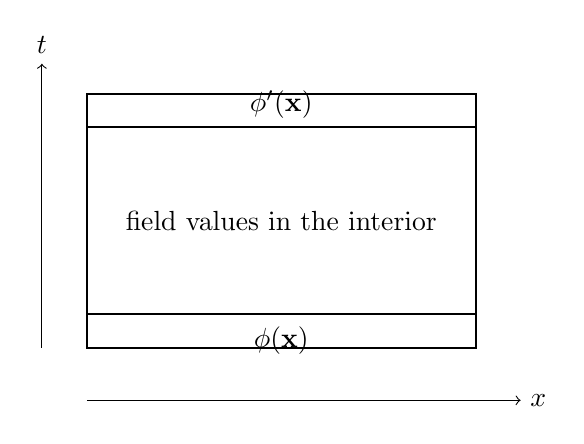
\begin{tikzpicture}[scale=0.95]
\draw[->] (-0.6,0) -- (-0.6,3.8) node[above] {$t$};
\draw[->] (0,-0.7) -- (5.8,-0.7) node[right] {$x$};
\draw[thick] (0,0) rectangle (5.2,3.4);
\draw[thick] (0,0.45) -- (5.2,0.45);
\draw[thick] (0,2.95) -- (5.2,2.95);
\node at (2.6,0.1) {$\phi(\mathbf{x})$};
\node at (2.6,3.25) {$\phi'(\mathbf{x})$};
\node at (2.6,1.7) {field values in the interior};
\end{tikzpicture}
\caption{The field-theory analog of fixed endpoints: initial and final field configurations on two time slices, with a spacetime region in between.}
\end{figure}

We may therefore phrase the classical field problem this way. Given \(\phi(\mathbf{x})\) initially and \(\phi'(\mathbf{x})\) finally, is there a field configuration in the slab between them? Classically the answer is yes, and the correct interpolating field is the one selected by the least-action principle. If we carry that out, the lecture reminds us, we recover partial differential equations such as Maxwell's equations.

\section{Particle Amplitudes and Feynman's Rule}

All right, now let us come back to quantum mechanics. The lecture makes this transition very explicitly. The quantum-mechanical object is no longer the trajectory itself, but the amplitude. We imagine a particle injected at a spacetime point \((x,t)\), we wait, and then we ask for the amplitude that a detector later finds it at \((x',t')\).

That amplitude is a complex number. The probability is not the amplitude itself, but its absolute square:
\begin{equation}
P=|\mathcal{A}|^2=\mathcal{A}\mathcal{A}^*.
\end{equation}
This point is stressed more than once in the lecture. The sum over paths gives the probability amplitude; only after multiplying by the complex conjugate do we get the probability.

Feynman's rule is then stated in its essential form. For each possible particle trajectory we compute the action and assign to that trajectory the phase
\begin{equation}
e^{-iS/\hbar}=e^{-\frac{i}{\hbar}\int \mathcal{L}\,dt}.
\end{equation}
The lecture remarks that Planck's constant has the units of action, so what appears in the phase is the action measured in units of \(\hbar\). That is where quantum mechanics enters. One may later set \(\hbar=1\), as the lecture briefly notes, but it is better to keep it explicit here.

\begin{figure}[h]
\centering

\includegraphics[width=0.70\textwidth]{lecture_10_figure_04.png}

\begin{tikzpicture}[scale=0.9]
\draw[->] (0,0) -- (4.8,0) node[right] {$x$};
\draw[->] (0,0) -- (0,3.2) node[above] {$t$};
\draw[thick] (1.0,0.6) .. controls (1.5,2.4) and (2.7,2.8) .. (2.3,1.3)
                     .. controls (2.0,0.6) and (3.0,0.9) .. (4.0,2.5);
\fill (1.0,0.6) circle (2pt);
\fill (4.0,2.5) circle (2pt);
\end{tikzpicture}
\caption{Phase factor associated with a particle path. The lecture frame is kept, and the small path sketch is redrawn schematically below.}
\end{figure}

The amplitude is the sum over all such paths:
\begin{equation}
\mathcal{A}(x,t\to x',t')=\sum_{\text{paths}} e^{-iS/\hbar}.
\end{equation}
The lecture adds one restriction in the nonrelativistic case: we do not allow the path to loop backward in time. But the decisive point is that every possible path contributes. In the lecture's language these are ``possible roots'' or ``possible trajectories,'' not only solutions of Newton's equations.

It is also worth preserving one of the lecture's small but revealing remarks. Why exponential? Because amplitudes for successive little steps multiply. That is the multiplicative structure which later becomes the product over spacetime cells.

\subsection{Question \& Answer}

\paragraph{Question.} If every contribution is an exponential of \(i\) times something, then each contribution has magnitude one. Why does the sum not blow up?

\paragraph{Answer.} Because the contributions are phases, not positive numbers. They live on the unit circle in the complex plane, and they oscillate. The point is not that the terms get smaller. They do not. The point is that they cancel. If phases are spread around the circle, their sum can be small or even vanish.

\paragraph{Question.} Then how does classical mechanics emerge at all?

\paragraph{Answer.} The lecture's answer is that the paths near the classical path cancel least. Most paths interfere destructively, but near a path of stationary action the phase changes more slowly, so there is less cancellation. In the lecture's spoken idiom these are the paths of minimum action. That is how the classical description reappears from the quantum one.

\section{From Trajectories to Field Histories}

We now make the decisive translation into field theory. One is tempted to ask for the amplitude to go from one spacetime event to another in the field case as well, but the lecture stops that thought immediately. No, the trajectory is replaced by a history.

A history means the values of the fields throughout the spacetime region between the initial and final slices. So we begin with an initial configuration \(\phi(\mathbf{x})\) and a final configuration \(\phi'(\mathbf{x})\). These are not numbers at two points; they are two functions over space. The amplitude is obtained by summing over all field histories that interpolate between them:
\begin{equation}
\mathcal{A}\big[\phi(\mathbf{x})\to \phi'(\mathbf{x})\big]
=\sum_{\text{histories}} e^{-iS[\phi]/\hbar},
\qquad
S[\phi]=\int d^4x\,\mathcal{L}(\phi,\partial_\mu\phi).
\end{equation}

The lecture is careful to say that this is an idealization. We do not literally prepare the field at every point in space and later measure it at every point in space. But as a conceptual question it is exactly the correct analog of the particle question. Every possible history one can imagine carries an action. Whether or not it is a true classical solution, it contributes a phase. The total amplitude is the sum of all those phases.

At this stage the object has been named, but not yet made usable. The lecture now changes register. He says, in effect: I am not going to derive the next step rigorously; I only want to show what this object is before I tell you how it is used in practice.

\section{Discretizing Spacetime to Make Sense of the Path Integral}

The practical step is to divide spacetime into little cells. This is how the lecture gives concrete meaning to the path integral. Instead of a continuum field, we think of one field value in each cell, and at the end one imagines letting the cell size go to zero.

This is also where the lecture explicitly corrects its earlier oversimplification. The previous heuristic had been ``one plus the Lagrangian'' in each cell. Then comes the correction: it is not the Lagrangian itself, but the action in each cell, that matters. If the cell has spacetime volume
\[
a^4=\Delta x\,\Delta y\,\Delta z\,\Delta t,
\]
then the action in the \(i\)-th cell is
\begin{equation}
A_i=\mathcal{L}_i\,a^4.
\end{equation}
Because the cell is small, \(A_i\) is small. This motivates the familiar approximation
\begin{equation}
1+\epsilon \approx e^\epsilon,
\end{equation}
and the lecture even writes out the beginning of the power series:
\begin{equation}
e^\epsilon=1+\epsilon+\frac{\epsilon^2}{2!}+\frac{\epsilon^3}{3!}+\cdots .
\end{equation}
But the lecture immediately sharpens the point: the cleaner and more correct thing is to use the exponential from the beginning.

Now replace the spacetime integral in the action by a sum over cells. Then
\begin{equation}
e^{-\frac{i}{\hbar}\sum_i A_i}
=
\prod_i e^{-iA_i/\hbar}.
\end{equation}
This is the practical content of the step. Before we sum over histories, the weight for one fixed history is an exponential of a sum, hence a product of exponentials, one factor for each cell.

\begin{figure}[h]
\centering
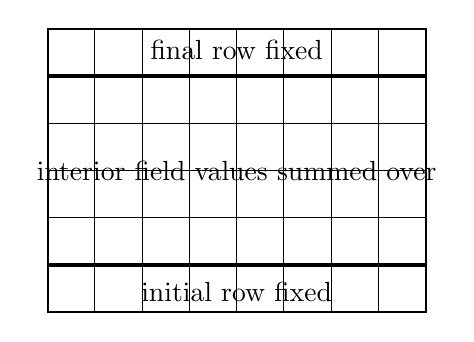
\begin{tikzpicture}[scale=0.75]
\draw[step=0.8,thin] (0,0) grid (6.4,4.8);
\draw[thick] (0,0) rectangle (6.4,4.8);
\draw[very thick] (0,0.8) -- (6.4,0.8);
\draw[very thick] (0,4.0) -- (6.4,4.0);
\node at (3.2,0.35) {initial row fixed};
\node at (3.2,4.45) {final row fixed};
\node at (3.2,2.4) {interior field values summed over};
\end{tikzpicture}
\caption{A lattice-like spacetime discretization. The first and last rows encode the boundary data; the interior is summed over.}
\end{figure}

We may therefore write the discrete version of the path integral schematically as
\begin{equation}
\mathcal{A}\big[\phi_{\mathrm{in}}\to\phi_{\mathrm{out}}\big]
=
\sum_{\{\phi\}_{\mathrm{interior}}}
\prod_i e^{-iA_i/\hbar}.
\end{equation}
The first and last rows are held fixed. The sum is over all assignments of field values in the interior cells. The lecture emphasizes that the product is first formed for a given history, and only then do we sum over histories.

\subsection{Question \& Answer}

\paragraph{Question.} Must the histories be continuous, or at least approximately continuous?

\paragraph{Answer.} No. The lecture answers this emphatically. Once spacetime is divided into cells, continuity is not the right requirement. We simply assign field values to the cells and sum over all assignments. There is no restriction to smooth or nearly smooth histories. Quantum fields, as the lecture puts it, jiggle a great deal.

\paragraph{Question.} Then what becomes of derivatives?

\paragraph{Answer.} We do not sum over derivatives as independent variables. We sum over field values. Derivatives are then represented by differences between neighboring cells:
\begin{equation}
\partial_\mu\phi(x)\ \longrightarrow\ \frac{\phi(x+\hat\mu)-\phi(x)}{a}.
\end{equation}
The lecture does not fix a single convention in detail. The point is only that derivatives are reconstructed from neighboring field values.

\paragraph{Question.} And how is this handled in actual calculations?

\paragraph{Answer.} Here the lecture briefly points toward lattice quantum field theory as a mature subject in its own right. The computational technology is not the subject of the chapter, but the motivational beat matters: the lattice is not merely a hand-waving picture. It is a real way of defining and calculating with the theory.

\section{Reading Particle Propagation Out of the Quadratic Terms}

Now let us go back once more, this time from fields to particles. The lecture says explicitly that quantum fields are shorthand for creation and annihilation operators. Thus a product of fields in neighboring boxes may be read as annihilating a particle in one box and creating it in another. That is how local terms in the Lagrangian become particle motion.

There is, however, one small correction to preserve. Not every term belongs to a single box. Derivative terms naturally belong to neighboring pairs of boxes. On the lattice a derivative becomes a difference, and the lecture insists that we are dealing with first derivatives only. Second-derivative terms are rejected as a bad idea. Thus the basic quadratic structure is neighbor-to-neighbor.

Schematically,
\begin{equation}
\bigl(\phi(x)-\phi(x')\bigr)^2
=
\phi(x)^2+\phi(x')^2-2\phi(x)\phi(x').
\end{equation}
The cross term \(\phi(x)\phi(x')\) is the one the lecture isolates as the source of propagation from one neighboring box to another. The same-site terms \(\phi(x)^2\) and \(\phi(x')^2\) already tell us that ``standing still'' is also built into the quadratic theory.

That is why the lecture focuses on a schematic nearest-neighbor sum of the form
\begin{equation}
\sum_{\langle x,x'\rangle}\phi(x)\phi(x').
\end{equation}
Then one expands the exponential:
\begin{align}
\exp\!\left[-i\sum_{\langle x,x'\rangle}\phi(x)\phi(x')\right]
&=
1
-i\sum_{\langle x,x'\rangle}\phi(x)\phi(x')
-\frac{1}{2!}\left(\sum_{\langle x,x'\rangle}\phi(x)\phi(x')\right)^2
+\cdots .
\end{align}
This is only a cautious schematic reconstruction. The lecture is using the expansion qualitatively. The precise coefficients multiplying the lattice terms are not the point here; the combinatorics of how paths are built is.

A single factor \(\phi(x)\phi(x')\) gives one elementary hop. If the initial and final points are already neighboring, that first-order term contributes directly, with the coefficient read off from the expansion. A two-step chain comes from the second-order term and carries the corresponding factorial and sign. In this way one sees the original path-integral idea reappearing inside the field-theory lattice expansion: long-distance propagation is assembled from local nearest-neighbor moves.

\begin{figure}[h]
\centering
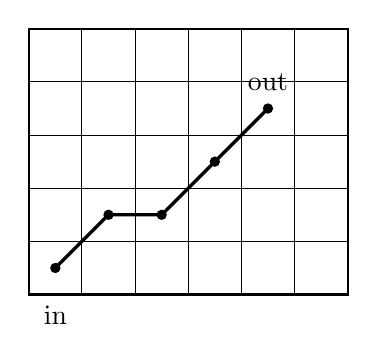
\begin{tikzpicture}[scale=0.75]
\draw[step=0.9,thin] (0,0) grid (5.4,4.5);
\draw[thick] (0,0) rectangle (5.4,4.5);
\fill (0.45,0.45) circle (2.5pt);
\fill (1.35,1.35) circle (2.5pt);
\fill (2.25,1.35) circle (2.5pt);
\fill (3.15,2.25) circle (2.5pt);
\fill (4.05,3.15) circle (2.5pt);
\draw[very thick] (0.45,0.45) -- (1.35,1.35) -- (2.25,1.35) -- (3.15,2.25) -- (4.05,3.15);
\node at (0.45,-0.35) {in};
\node at (4.05,3.6) {out};
\end{tikzpicture}
\caption{A schematic chain of nearest-neighbor hops. Higher-order terms in the expansion build long-distance propagation from local links.}
\end{figure}

There is one more rule the lecture treats almost as a commandment: no dangling ends, except where we explicitly put particles in at the bottom or take them out at the top. This is what forces local hop terms to join into full paths rather than floating fragments.

The mass term then adds a second kind of local rule:
\begin{equation}
\frac{1}{2}m^2\phi^2.
\end{equation}
This does not move the particle. It annihilates and recreates it at the same site, thereby weighting the path while leaving it in place. At the very end of the lecture Susskind returns to this point and notes that ``standing still'' comes from two places: from the same-site terms already contained in \((\phi(x)-\phi(x'))^2\), and from the explicit mass term as well.

\subsection{Question \& Answer}

\paragraph{Question.} How do local nearest-neighbor terms build a long-distance propagator without leaving illegal loose ends?

\paragraph{Answer.} By going to higher orders in the exponential expansion. A single nearest-neighbor term gives one hop. Two such terms can join into a two-step chain. Three such terms can make a longer chain, and so on. The contributing terms are precisely those in which all internal endpoints are paired off, leaving only the initial and final insertion points exposed.

\paragraph{Question.} What about motion backward in time?

\paragraph{Answer.} In the relativistic theory it is allowed, and the lecture presents two readings of the same picture. One may say the path literally goes backward in time, or one may read the same graph forward in time as a particle-antiparticle pair being created, with the antiparticle later annihilating the original particle. The lecture keeps both interpretations in play.

\begin{figure}[h]
\centering
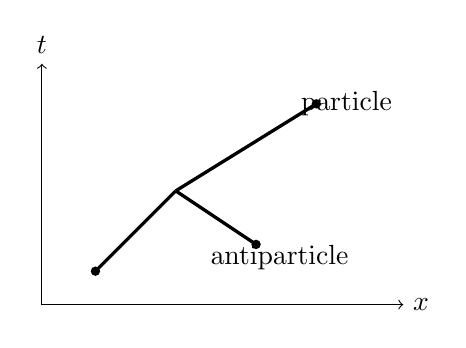
\begin{tikzpicture}[scale=0.85]
\draw[->] (0,0) -- (0,3.6) node[above] {$t$};
\draw[->] (0,0) -- (5.4,0) node[right] {$x$};

\draw[very thick] (0.8,0.5) -- (2.0,1.7);
\draw[very thick] (2.0,1.7) -- (3.2,0.9);
\draw[very thick] (2.0,1.7) -- (4.1,3.0);

\fill (0.8,0.5) circle (2pt);
\fill (3.2,0.9) circle (2pt);
\fill (4.1,3.0) circle (2pt);

\node at (4.55,3.0) {particle};
\node at (3.55,0.7) {antiparticle};
\end{tikzpicture}
\caption{A schematic backward-in-time segment reinterpreted as pair creation and annihilation. This is a pedagogical reading of the lecture, not a claim about exact board geometry.}
\end{figure}

\section{Interactions, Vertices, and the Perturbative Expansion}

Only now do we add the genuinely interacting terms. This order is important. The lecture first teaches us how the quadratic terms build propagation, and only after that does it allow particles to split and join.

A cubic term
\begin{equation}
g_3\phi^3
\end{equation}
can annihilate one particle and create two, or annihilate two and create one. In the operator language it can also create three or annihilate three. A quartic term
\begin{equation}
g_4\phi^4
\end{equation}
creates four-legged events: \(2\to2\) scattering, \(1\to3\), \(3\to1\), or fully virtual four-particle creation and annihilation processes. The lecture's point is not to catalog them abstractly, but to show that once higher powers appear in the Lagrangian, the lattice picture is no longer just a story of one particle hopping from box to box. It becomes a story in which particle number can change locally at a vertex.

\begin{figure}[h]
\centering
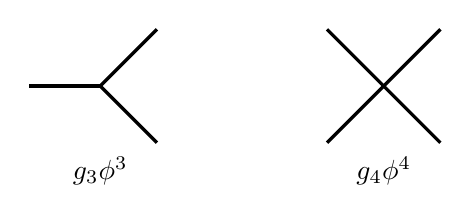
\begin{tikzpicture}[scale=0.9]
\draw[very thick] (0,0)--(1.0,0);
\draw[very thick] (1.0,0)--(1.8,0.8);
\draw[very thick] (1.0,0)--(1.8,-0.8);
\node at (1.0,-1.2) {$g_3\phi^3$};

\draw[very thick] (4.2,0.8)--(5.0,0);
\draw[very thick] (4.2,-0.8)--(5.0,0);
\draw[very thick] (5.0,0)--(5.8,0.8);
\draw[very thick] (5.0,0)--(5.8,-0.8);
\node at (5.0,-1.2) {$g_4\phi^4$};
\end{tikzpicture}
\caption{Schematic cubic and quartic vertices. These are clean pedagogical redrawings of the local processes described in the lecture.}
\end{figure}

From here the lecture widens rapidly. A one-particle propagator is no longer merely the sum of simple hop-by-hop paths. On the way, a cubic term may act and split the particle into two. One of those may later be reabsorbed. In the physical language of electrodynamics, an electron may emit a photon and later reabsorb it. Even that is only the beginning. The photon may split into an electron-positron pair, and so on. The full amplitude is the sum of all such allowed histories.

This is the right place to say clearly what the lecture means by the equivalence of Lagrangian language and Feynman-diagram language. The quadratic terms define propagators. The higher-order terms define vertices. A propagator is just a line between two points; a vertex is a point at which several lines meet. The diagrams are not extra physics added on top of the Lagrangian. They are a shorthand reading of the information already encoded in it.

Conservation laws are also recovered in this language. The lecture recalls that when one integrates a vertex over all time, energy conservation appears, and when one integrates over all space, momentum conservation appears. The same idea is applied here. If a process violates energy or momentum conservation, the sum over all possible spacetime positions of the relevant vertices cancels it out.

This is also where the lecture makes a sharp practical point about couplings. Every vertex contributes a power of the appropriate coupling. Thus, schematically,
\begin{equation}
\mathcal{A}_{\mathrm{diagram}}\propto g_3^{V_3}g_4^{V_4}\cdots .
\end{equation}
If the couplings are small, more complicated diagrams are suppressed, and perturbation theory has a chance to be useful.

A particularly clear worked example comes from quantum electrodynamics. The interaction between an electron and a photon is governed by the electric charge \(e\). The lowest-order electron-photon scattering amplitude contains two such vertices, so
\begin{equation}
\mathcal{A}_{\mathrm{QED,\,lowest}}\propto e^2.
\end{equation}
The corresponding probability, or cross section, scales as
\begin{equation}
P_{\mathrm{QED,\,lowest}}\propto e^4.
\end{equation}
The lecture immediately adds two important refinements. First, even at this order there is more than one diagram, so we must add the amplitudes of all graphs of the same order. Second, every extra complication in a QED diagram adds more powers of \(e\), and therefore produces smaller corrections when \(e\) is small.

So one must keep the order of operations straight:
\begin{equation}
\mathcal{A}_{\mathrm{total}}=\sum_r \mathcal{A}_r,
\qquad
P=\left|\sum_r \mathcal{A}_r\right|^2.
\end{equation}
We do not square each graph separately and add probabilities. We add amplitudes first and only then square. The cross terms are the interference terms, and they are part of the physics.

\subsection{Question \& Answer}

\paragraph{Question.} Where do the coupling constants come from?

\paragraph{Answer.} Sometimes symmetries relate them, but in general the lecture answers very plainly: their values come from experiment. The Lagrangian is partly governed by theory and symmetry, and partly by measured input.

\paragraph{Question.} Then why is the enormous sum over processes computationally useful?

\paragraph{Answer.} Because every extra vertex contributes another power of the coupling. If the coupling is small, higher-order graphs are progressively less important. This does not settle every mathematical question of convergence, and the lecture says so, but it explains why the perturbative expansion can work so well in practice.

There is also one late caution worth preserving. The lecture notes that the relation between fields and particles need not always be one-to-one. In weakly coupled theories particle language is natural, but more generally the field description can remain fundamental even when the particle interpretation becomes less sharp. Still, for the present course the Lagrangian is useful in both languages, and that dual usefulness is the real takeaway.

\section{Summary}

The lecture unfolds by repeated returns. We go back to classical least action in order to come forward to quantum amplitudes. For a particle, every path contributes a phase \(e^{-iS/\hbar}\). For a field, the path is replaced by a history, and the amplitude becomes a sum over all interpolating field configurations. To make that sum concrete, we divide spacetime into cells, attach an action to each cell, and rewrite the exponential of the total action as a product over the lattice. From the quadratic terms we read propagation and same-site weighting; from higher powers such as \(\phi^3\) and \(\phi^4\) we read splitting, joining, and scattering vertices. In this way the same Lagrangian can be read as a field-history action or as a catalogue of propagators and vertices. That is why the lecture can now move on, in the next stage of the course, to the world of actual particles.